\section{Methods}\label{sec:methods}

We adapt SMiRL to the problem of optimizing a price-serving agent for energy demand response. 
We will briefly explain the baseline Proximal Policy Optimization (PPO).
We will then describe the simulation environment we test this in. 

\subsection{Environment}

We summarize an OpenAI gym environment modeled after an environment to simulate demand response in office buildings \cite{spangherofficelearn}.  
Each step in the environment is a day, where the agent proposes prices to office workers, 
who modify their energy consumption behaviors in order to achieve the lowest cost of energy possible, 
which the controller then takes as their respective rewards. 
Each simulated person has a deterministic response to the points that are offered to them.

\begin{figure}
\centerline{
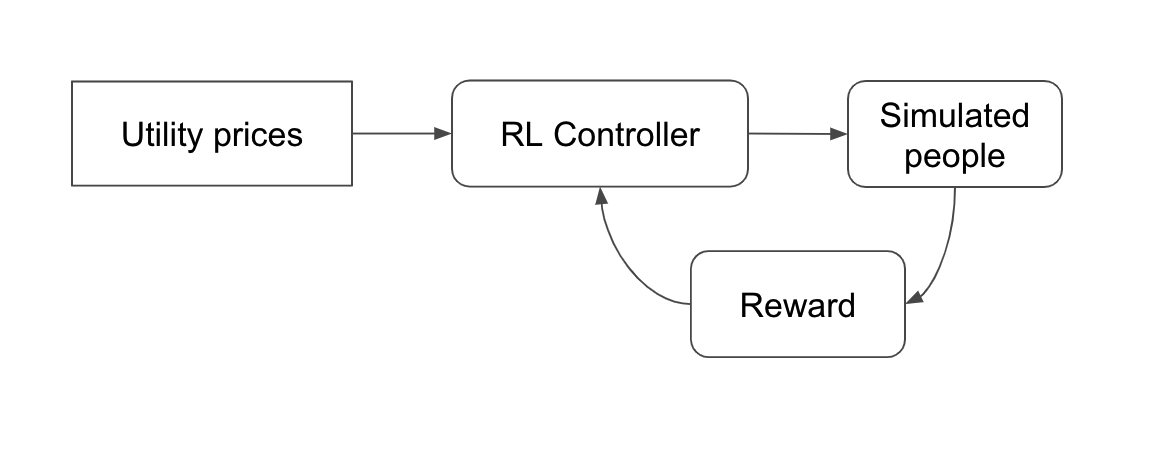
\includegraphics[width=0.9\linewidth]{graphics/RLcontroller.png}
}
\caption{Reinforcement Learning Control Flow} \label{fig:RLcontroller}
\end{figure}

Can an RL agent learn to provide optimal price signals by implicitly predicting causal factors? 
Our search space is simple enough to efficiently cover with an entropy maximizing agent, and so we employ a Proximal Policy Optimization (PPO) architecture. 
We use Ray's RLLib PPO algorithm.
The reward for the price-setting agent is 
$$ r_{\text{energy}} = \log(d^tg) $$
where $d$ is the demand of the person it studies, and $g$ is the grid pricing. 
We use parameters of learning rate $ 
\alpha = 0.003$, batch size of $ 256 $, training stochastic gradient descent 
minibatch of $ 32 $, clip parameter $ 0.3 $ and all other parameters were RLLib
PPO defaults. 
For other implementation choices, please see our Github\footnote{Our Github may be found at the following link: \url{https://github.com/Aphoh/temp_tc}.}

\subsection{SMiRL Reward Formulation}
A SMiRL agent recieves an auxiliary reward for 
experiencing familiar states based on an updating distribution of states it has experienced. 
This is exactly equivalent to learning a policy with the lowest entropy. 
Assuming we have a fully-observed controlled Markov process (CMP) with state $ s_t $ and action $ a_t $
at time $ t $, and $ p(s_0) $ as the initial state distribution, and transition probabilities 
$ T(s_{t+1} | s_t, a_t) $, the agent learns a policy $ \pi_\phi (a | a) $ parameterized by 
$ \phi $. 
As described earlier, we keep track of an estimated state marginal $ p_{\theta_{t-1}} (s_t) $ 
for the actual state marginal $ d^{\pi_\phi} (s_t) $. 
As usual we denote entropy of a state $ s_t $ by $ \entropy{s_t} $. 
The entropy can then be calculated by the marginal as 
\begin{align}
    \sum_{t=0}^{T} \mathcal{H}\left(\mathbf{s}_{t}\right)
    &= -\sum_{t=0}^{T} \mathbb{E}_{\mathbf{s}_{t} \sim d^{\pi} \phi\left(\mathbf{s}_{t}\right)}\left[\log d^{\pi_{\phi}}\left(\mathbf{s}_{t}\right)\right] \\
    &\leq-\sum_{t=0}^{T} \mathbb{E}_{\mathbf{s}_{t} \sim d^{\pi} \phi\left(\mathbf{s}_{t}\right)}\left[\log p_{\theta_{t-1}}\left(\mathbf{s}_{t}\right)\right] 
\end{align}
We bound (1) by the entropy of an estimated marginal $ p_{\theta_{t-1}} $ in (2).
Minimizing the right side bound is then equivalent to maximizing an RL objective with reward 
$ r_{\text{SMiRL}}(s_t) = \log p_{\theta_{t-1}} (s_t)  $
We note that the optimal policy must also consider future changes to $ p_{\theta_{t-1}} (s_t) $
since the distribution of visited states changes at each step. 
To account for this we use an augmented MDP that captures this notion. \citep{smirl}
We note that in our implementation of SMiRL, $ p_{\theta_t} (s) $ is normally distributed. 
To construct the augmented MDP we include sufficient statistics for $ p_{\theta_t} (s)$ 
in the state space such as the paramaeters of our normal distribution and the number of states 
seen so far. 

\subsection{SMiRL Implementation}
SMiRL is simply implemented in our existing OpenAI socialgame environment. 
We introduce SMiRL into our existing socialgame environment by initializing a 
buffer that tracks the agent's observed states and computes an estimated state marginal $ p_{\theta_t} $. 
As noted earlier, in the augmented MDP the state space also contains the number of observed states and this information is stored in the buffer as well. 
At each step in our simulation we add newly observed states to our buffer, and update $p_{\theta_t}$. The agent then adjusts the its policy based on the combined reward. 

We notice that since $ p_{\theta}(s) $ is modeled as an independent Gaussian for each dimension (hour) in the observation (consumption for a day), 
then the SMiRL reward is expressed as 
$$ r_{\text{SMiRL}}(s_t) = - \sum\limits_i \left( \log \sigma_i + \frac{(s_i - \mu_i)^2}{2\sigma_i^2} \right)  $$
where $ \mu_i $ and $ \sigma_i$ are the sample mean and standard deviation from our state marginal 
and $ s_i $ is the $ i^{th}$ feature ($ i^{th} $ hour of day) of $ s $ \citep{smirl}.
With this formulation we can efficiently calculate the SMiRL reward from our buffer. 

\subsection{SMiRL as an Auxilary Reward}
We use SMiRL as an auxilary reward to provide faster learning and more stable outputs. 
We achieve this by calculating the SMiRL reward $ r_{\text{SMiRL}} $ as described in the previous section, and applying a SMiRL weight $ \alpha $ to it and then using the sum with our usual energy 
reward $ r_{\text{energy}} = \log(d^tg) $. This gives us a combined reward of 
\begin{equation}
    r_{\text{combined}} = r_{\text{energy}} + \alpha r_{\text{SMiRL}}
\end{equation}
and it is this reward that we use to train the RL agent. 
In our simulations, we found the optimal SMiRL weight $ \alpha $  to be around $ \alpha = 0.12$ after 
hyperparameter tuning. 
We will discuss the exact results of various SMiRL weights in Section \ref{sec:results}. 
